\documentclass[UTF8]{ctexart}
\usepackage{ulem}
\usepackage[scale=0.8]{geometry}
\usepackage{color}
\usepackage{graphicx}
\usepackage{wrapfig}

\usepackage[backend=bibtex, style=gb7714-2015, sorting=ynt]{biblatex}
\addbibresource{ref.bib}

\title{\textbf{巴勒斯坦 - 以色列政治、历史相关谣言及辟谣}}
\author{XYCode}
\date{修订版本:0.0.1-rev.1+20240511}

\begin{document}
    \maketitle

    \tableofcontents

    \section*{前言}
        这篇文档的目的是\textbf{收集和辟谣}关于巴勒斯坦-以色列政治历史的谣言,而\textbf{不代表}任何政治观点。
        
        我们知道,巴勒斯坦 - 以色列之间长期以来一直充满了紧张局势和复杂的政治问题,因此谣言也经常在其中传播。我们希望通过澄清事实,帮助人们更好地理解这个地区的历史和现状。

        首先,我们要明确的是,谣言和不实信息可能会导致误解和进一步的紧张局势,导致公众对双方产生误解。因此,我们呼吁大家对获取的信息保持警惕,尤其是对于历史、政治关系及其复杂的巴勒斯坦地区。

        关于巴勒斯坦和以色列的历史,有许多传言经常出现,比如关于领土归属、历史解释、双方立场等等。我们将努力在这里澄清一些常见的谣言,并提供事实依据。
    
    \section{巴勒斯坦 - 以色列冲突(2024)}
        \subsection{(不利于) 巴勒斯坦方面的谣言整理}
            \subsubsection{哈马斯是恐怖组织}
                不同国家对于哈马斯的性质定义不同,这种差异体现了政治立场和国际关系的复杂性。对于哈马斯到底是恐怖组织还是合法的政治实体,不同国家和组织之间存在着激烈的争议。

                目前,安理会、伊朗、土耳其、中华人民共和国、多数阿拉伯国家、俄罗斯承认其\textbf{抵抗组织}的定位。其中卡塔尔王室、伊朗为哈马斯提供了资金和武器支持。\cite{wiki:哈马斯}

                而多数西方国家,例如以色列、美国、加拿大、欧盟、英国、澳大利亚等则将其认定为\textbf{恐怖组织}。\cite{wiki:哈马斯}

                无论如何,我们都必须谴责哈马斯对于以色列平民的无差别袭击,也必须肯定其为保卫巴勒斯坦、争取民族独立所作出的斗争。
            
            \subsubsection{哈马斯是在野党/非法党派/军阀}
                巴勒斯坦于2006年举行了第二次立法委选举,哈马斯在立法委132个席位中获得约70个席位,成为巴勒斯坦立法会多数党。巴勒斯坦总理赖内阁递交了辞呈,巴勒斯坦解放组织阿巴斯授权在立法会选举中获多数席位的政党组阁。\cite{光明网2006哈马斯赢得大选}

            \subsubsection{法塔赫是巴勒斯坦人民的唯一代表}
                巴勒斯坦解放组织(PLO)是巴勒斯坦人民的合法代表,巴勒斯坦民族解放运动(法塔赫)是PLO的一个党派。\cite{外交部2019巴勒斯坦国家概况}

                巴勒斯坦自治政府(巴勒斯坦民族权利机构)是PLO下属的一个机关,巴勒斯坦全国委员会(立法会)是该国最高权力机关。\cite{外交部2019巴勒斯坦国家概况}

                % PLO 标志
                \begin{figure}[htbp]
                    \centering
                    
\includegraphics[height=5cm]{./images/PLO-logo.jpg}
                    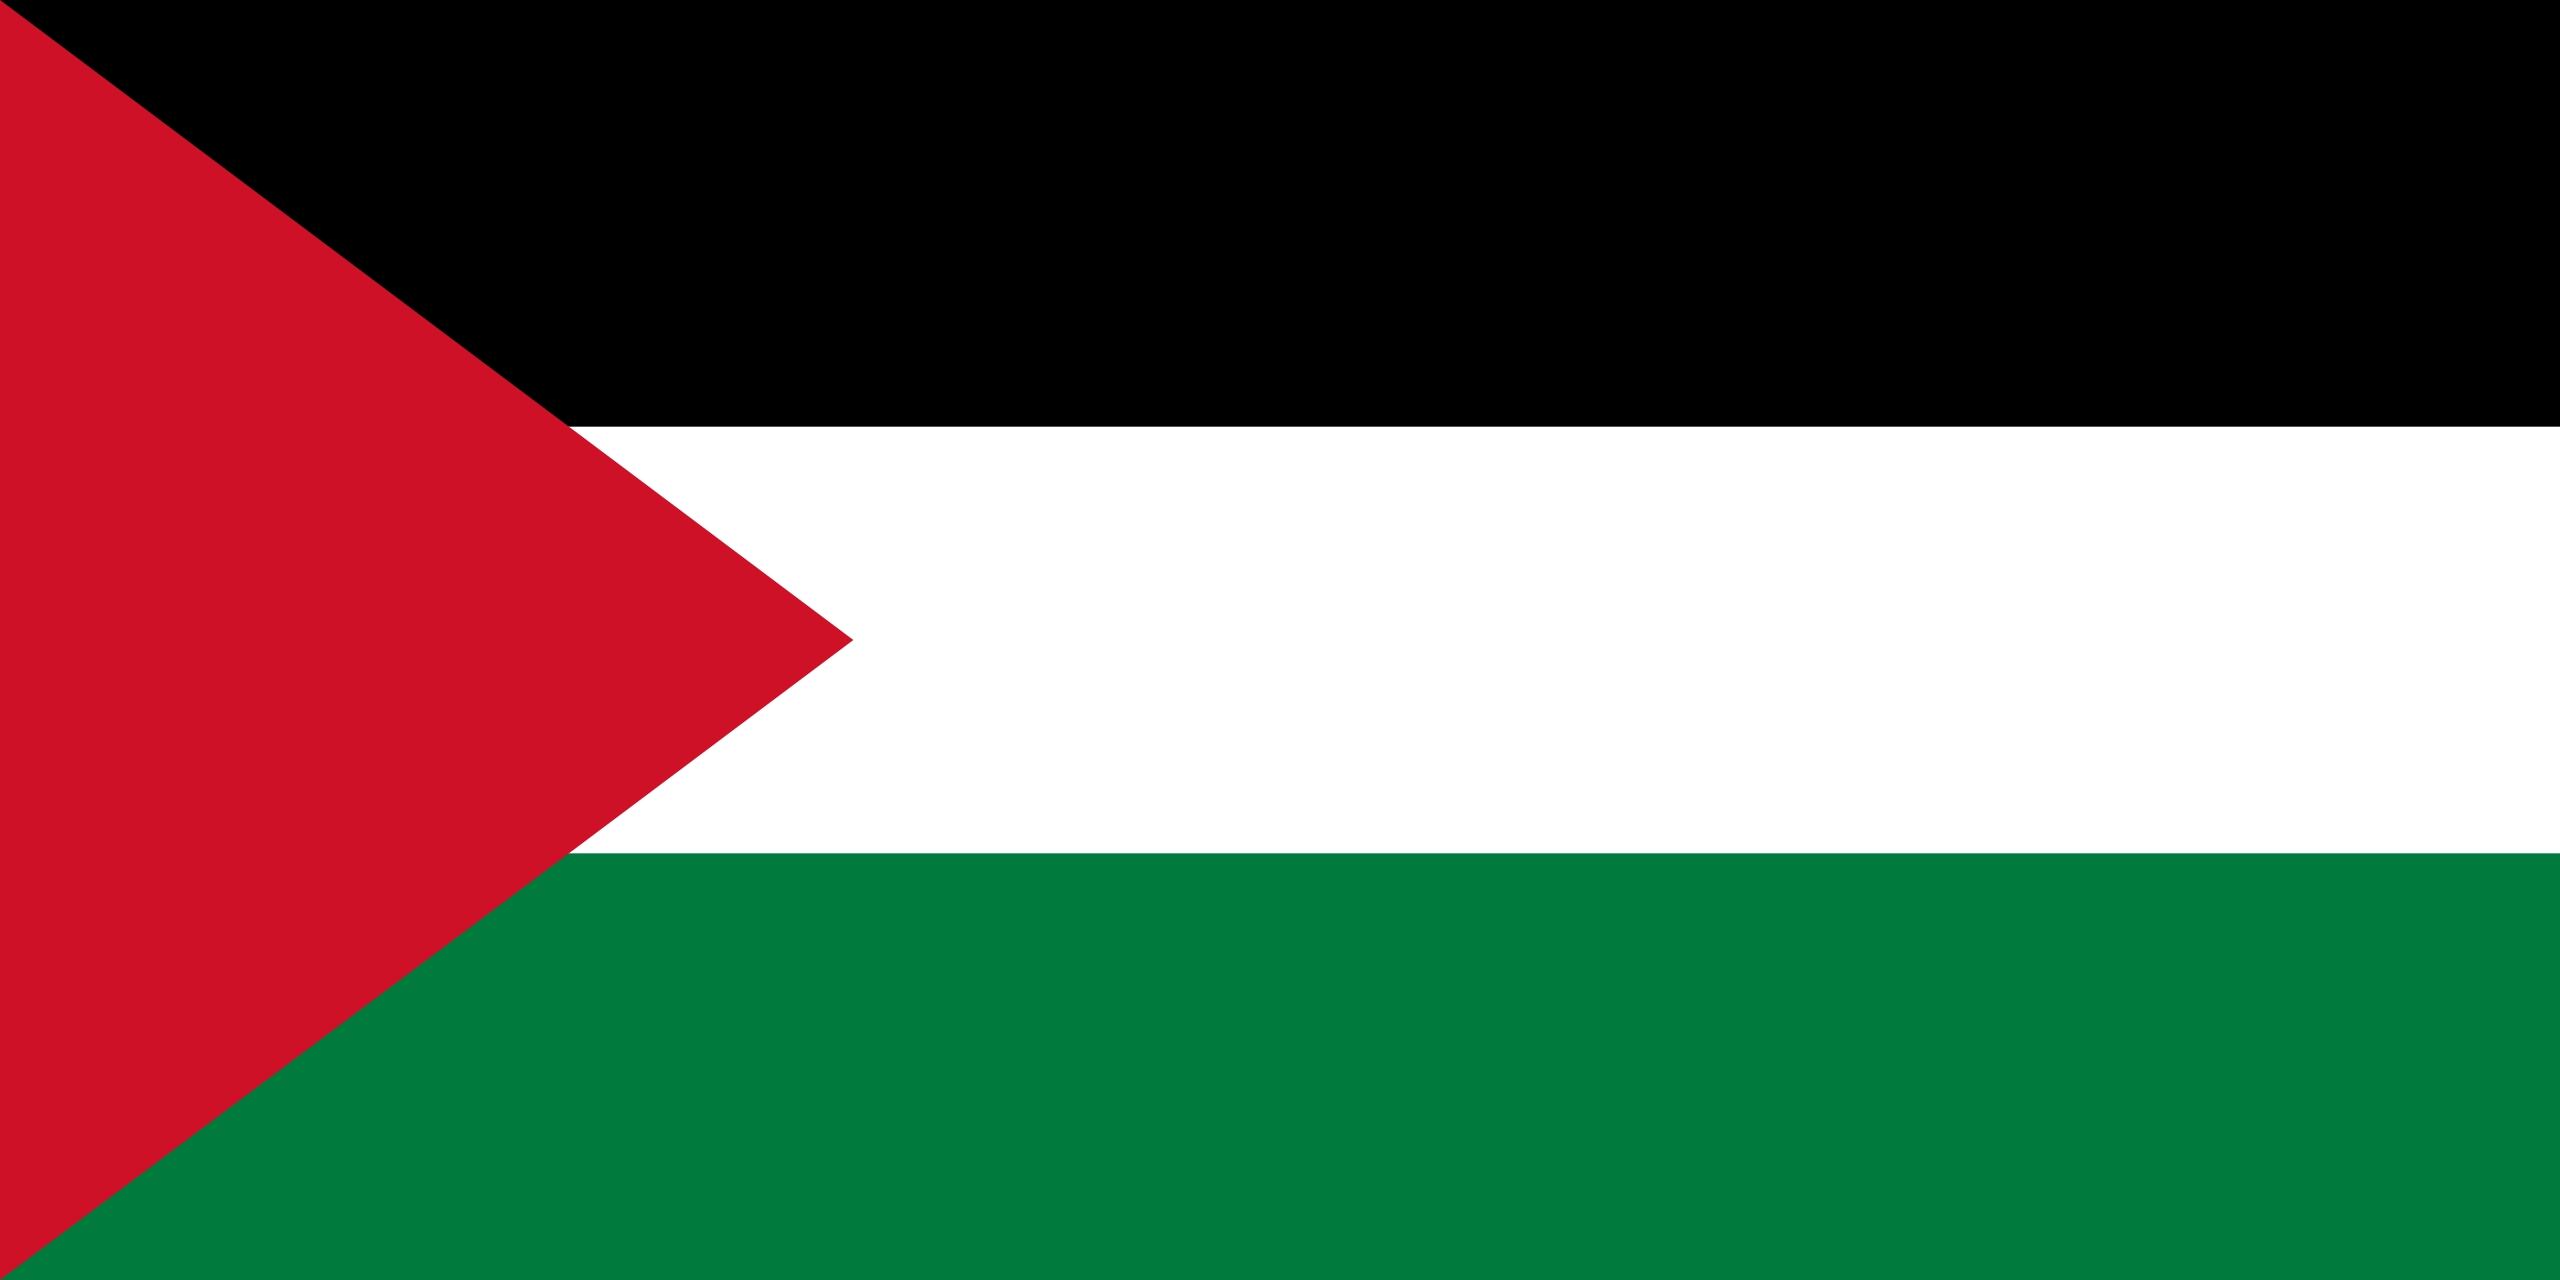
\includegraphics[height=5cm]{./images/PLO-flag.jpg}
                    \caption{巴勒斯坦解放组织标志和旗帜(暨巴勒斯坦国徽和国旗)}
                \end{figure}
            
            \subsubsection{哈马斯毫无理由的发动了阿克萨洪水行动}
                “阿克萨洪水”这一行动名称就暗示了其的背景,即\textbf{阿克萨清真寺冲突事件}。\cite{央视新闻2023阿盟就阿克萨清真寺冲突事件召开紧急会议,谴责以方行为}

                2023年4月5日,以色列警方凌晨进入了伊斯兰教圣地阿克萨清真寺并与巴勒斯坦民众发生暴力冲突,造成15名巴勒斯坦人受伤,350多名巴勒斯坦人被逮捕。事后,加沙地带武装组织向以色列境内发射了十多枚火箭弹。随后,以军对巴勒斯坦伊斯兰抵抗运动(哈马斯)在加沙地带的多个军事设施发动空袭。\cite{央视新闻2023阿盟就阿克萨清真寺冲突事件召开紧急会议,谴责以方行为}

                \begin{figure}[htbp]
                    \centering
                    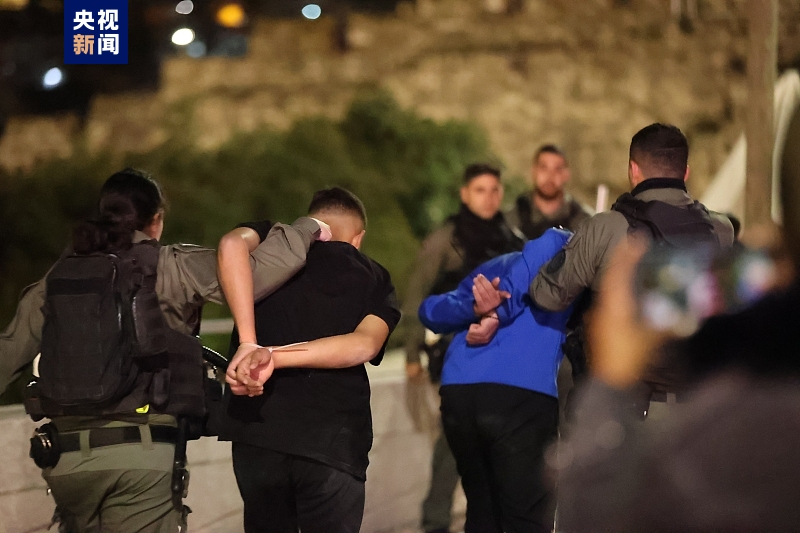
\includegraphics[width=0.4\textwidth]{images/以色列军警逮捕巴勒斯坦人.jpg}
                    \caption{以色列军警逮捕巴勒斯坦人 \footnotesize 央视新闻 图}
                \end{figure}

            \subsection{哈以冲突}
                {\small 维基百科关于阿克萨洪水行动的词条着重强调了\textbf{哈马斯被西方国家列为恐怖组织},而忽略了大多数国家将其定为抵抗组织的事实,并大量使用了\textbf{哈以冲突}一词。
                
                鉴于其公然将台湾地区列为国家的丑陋行径,我们\textbf{不推荐}各位使用维基百科来了解巴以冲突的相关信息。本文中引用自其的信息均已查实。}

                哈以冲突是语言学的刻意为之,是故意生造出的中文词。中华人民共和国的官方媒体均使用巴以冲突一词来代指\textit{巴勒斯坦、以色列冲突(The Israeli Palestinian Conflict)},而非使用哈以冲突。

                哈以冲突一词将巴勒斯坦替换为了哈马斯,暗示这并非国与国之间的冲突,而是巴勒斯坦党派和以色列国家之间的冲突。这一词的根本性错误在于其强调了巴勒斯坦方面只有哈马斯参战,从而可以塑造\textit{哈马斯不得民心}的形象,而事实是\textbf{\dotuline{有多个}巴勒斯坦党派在同以色列国防军交火}。

                巴勒斯坦联合作战指挥室(阿拉伯文罗马化:Ghrftāl mlyātālmshtrkh),也被称为巴勒斯坦抵抗派联合战斗室(阿拉伯文罗马化:Alghrftālmshtrktlfṣā lālmqāwmtālflsṭynyh),是加沙地带巴勒斯坦武装派别的联合战斗前线。它包括来自各种背景和意识形态的武装组织,既有伊斯兰主义者、社会主义者、民族主义者等右翼派别,也有左翼派别。\cite{wiki:Palestinian_Joint_Operations_Room}

                哈马斯、巴勒斯坦伊斯兰圣战组织(PIJ)、人阵、民阵、人民抵抗委员会、纳赛尔·萨拉赫·丁旅、圣战者旅、前法塔赫军事组织阿克萨烈士旅等均参加了巴勒斯坦联合作战指挥室,形成了统一战线。\cite{wiki:Palestinian_Joint_Operations_Room}

        \subsection{(不利于) 以色列方面的谣言整理}
            \subsubsection{以色列全民皆兵,因此不存在平民}
                以色列法律规定,以军每年征兵3次。所有公民(非犹太裔女性和所有阿拉伯裔男性除外),除宗教和健康原因,不分男女,年满18岁必须服兵役,高中毕业先当兵后上大学,以便将当年$90\%$以上的适龄男子和$50\%$以上的适龄女子征集服役。\cite{中国国防报2020全民皆兵的以色列战争动员模式}
            
            \subsubsection{以色列对于\uline{巴勒斯坦地区}的领土索取毫无依据}
                犹太人祖先曾在巴勒斯坦地区生活过,这并不是毫无依据的。现今世界广泛支持“两国方案”,即巴勒斯坦、以色列双方均建立以耶路撒冷为首都,主权完整的两个国家。
                
                现今世界广泛支持该方案,包括巴勒斯坦伊斯兰抵抗运动(哈马斯)、巴勒斯坦民族解放运动(法塔赫)、解放巴勒斯坦人民阵线(人阵)\footnote{巴勒斯坦马克思、列宁主义党派}、解放巴勒斯坦民主阵线(民阵)\footnote{巴勒斯坦毛泽东主义党派}在内的多个巴勒斯坦党派均支持该方案。

        \subsection{中立性谣言整理}
        
        \subsection{种族主义/民族主义/反犹主义/纳粹主义相关谣言整理}
            \subsubsection{反以犹太人是所谓“风险对冲”}
                以民族/种族来将人粗暴的划分是极其不可取的行为,无论哪个民族/种族,都有真正善良的人。例如在抗日战争中帮助八路军的日本共产党员\textit{德田球一}、德国人\textit{约翰·拉贝}。

                哈瑞迪教派对以色列的存在持有坚决反对的立场。他们认为以色列国家的建立是违背上帝的意愿的,因为根据他们对经文的解释,犹太人应该等待弥赛亚的到来,而不是依靠自己的力量建立国家。他们相信,只有在弥赛亚降临时,才能够实现真正的犹太民族复兴。\cite{半岛电视台2023哈瑞迪从边缘走向中心}

                也有出于对巴勒斯坦人同情而选择发声的犹太人:耶鲁大学支持巴勒斯坦学生游行的发言人是犹太人\cite{bilibili:巴勒斯坦游行犹太人发言人2024};组织\textit{犹太和平之声}在美国组织了多场抗议活动,其中包括一场冲击美国国会大厦的抗议。
    \printbibliography
\end{document}